\documentclass[10pt]{beamer}

%%%
% PREAMBLE FOR THIS DOC 
%%%
%https://tex.stackexchange.com/questions/68821/is-it-possible-to-create-a-latex-preamble-header
\usepackage{/Users/miw267/Repos/latex_preamble/beamer_preamble}

\usetikzlibrary{matrix}


%%% TRY TO RESHOW TOC AT EACH SECTION START (with current section highlighted)
% Reference: https://tex.stackexchange.com/questions/280436/how-to-highlight-a-specific-section-in-beamer-toc
\newcommand\tocforsect[2]{%
  \begingroup
  \edef\safesection{\thesection}
  \setcounter{section}{#1}
  \tableofcontents[#2,currentsection]
  \setcounter{section}{\safesection}
  \endgroup
}


%%%% HERES HOW TO DO IT CORRECTLY
% FIRST IN .STY FILE, DO
%\usetheme[sectionpage=none]{metropolis}
% THEN AT EACH SECTION DO
%\begin{frame}{Outline}
%  \tableofcontents[currentsection]	
%\end{frame}



%\setbeamertemplate{navigation symbols}{}
%\setbeamertemplate{footline}[frame number]{}

\newcommand{\leastElement}{s}

%%%
% DOCUMENT
%%%

\begin{document}

%\maketitle

%% Title page frame
%\begin{frame}
%    \titlepage 
%\end{frame}





\title{10/12/2026: Smallest Counterexample}
\author{CSCI 246: Discrete Structures}
\date{Textbook reference: Sec 21, Scheinerman}

\begin{frame}
    \titlepage 
\end{frame}


\begin{frame}

%\begin{myredbox}[title=\text{Announcements}]
%\begin{itemize}
%\item Please sign the attendance sheet.
%\end{itemize}
%\end{myredbox}
%
%
%\vfill 

\begin{myyellowbox}[title=Today's Agenda]
\begin{itemize}
\item ($\approx$ 30 min)  Mini-lecture
\item ($\approx$ 20 min) Group exercises	
\end{itemize}
\end{myyellowbox}
%\vfill 

\end{frame}



\begin{frame}{The Well-Ordering Principle}
\only<1->{In today's class, we'll use the following \textbf{axiom}.}
\vfill 
\only<2->{\begin{mybluebox}[title=\text{Axiom: The Well Ordering Principle}]
Every non-empty set of natural numbers contains a least element.
\end{mybluebox}
}
\vfill 
\only<3->{Seems pretty intuitive, right!?}
\vfill

\only<4-5>{
\begin{mygreenbox}[title=\text{Example 1}]

Let 
\[ S = \set{n \in \mathbb{N} : n^2 > 50}.\]
This set is a nonempty subset of the natural numbers. By the well-ordering principle, $S$ contains a least element: \only<4>{\alert{???}}\only<5>{\textbf{8.}}
\end{mygreenbox}
}

\only<6-7>{
\begin{mygreenbox}[title=\text{Example 2}]
Let 
\[ P = \set{x \in \mathbb{N} : x \text{ is prime}}.\]
This set is a nonempty subset of the natural numbers. By the well-ordering principle, $P$ contains a least element:  \only<6>{\alert{???}.}\only<7>{\textbf{2.}}
\end{mygreenbox}
}

\end{frame}


\begin{frame}{Smallest counterexample: the idea}

Smallest counterexample is new proof technique.  \pause Here we prove a claim using \alert{proof by contradiction.}
\pause 
\vfill
At a high level, the argument goes like this:
\begin{itemize}
\item Notice: If there exists a counterexample, there must be a minimal counterexample. \pause 
\item Show: The minimal counterexample produces a contradiction. \pause 
\item Conclude: The claim holds!	
\end{itemize} 
	
\end{frame}


\begin{frame}{Proof by smallest counterexample: A data science example}
\footnotesize

\colorbox{yellow!30}{\textbf{Setting.}} Data often arrives as a \textbf{stream} (sensor readings, web logs, a file too big for memory).  We can't store everything and then average, so we keep a \textbf{running mean}, updating it as each point $x_n$ arrives:
\[ \mu_1 = x_1, \qquad \mu_n = \mu_{n-1} + \frac{x_n - \mu_{n-1}}{n} \quad \text{for } n \geq 2. \]

\pause
\vfill
\begin{mybluebox}[title=\text{Claim.}]
For every positive integer $n$, the running mean equals the true mean:
\[ \mu_n = \frac{x_1 + x_2 + \cdots + x_n}{n}. \]
\end{mybluebox}

\pause
\vfill
\only<3->{\colorbox{green!30}{\textbf{Proof.}} Suppose not.  Then the set of $n$ for which the claim fails is a nonempty set of positive integers, so by the Well-Ordering Principle it has a \textbf{smallest element} $s$.}
\begin{itemize}
\item<4-> $s \neq 1$, since $\mu_1 = x_1 = \frac{x_1}{1}$.  %So $s-1 \geq 1$.
\item<5-> Since $1 \leq s-1 < s$, the claim \textbf{holds} for $s-1$:  \quad $(s-1)\,\mu_{s-1} = x_1 + \cdots + x_{s-1}$.
\item<6-> So
\[ \mu_s = \mu_{s-1} + \frac{x_s - \mu_{s-1}}{s} = \frac{(s-1)\,\mu_{s-1} + x_s}{s} = \frac{x_1 + \cdots + x_{s-1} + x_s}{s}, \]
so the claim holds for $s$, which contradicts $s$ being a counterexample. $\blacksquare$ \end{itemize}

\only<7->{\colorbox{red!30}{\textbf{Why care?}} \scriptsize  We've proven a one-pass streaming algorithm correct for \textit{every} input length. \greencheck}

\end{frame}

%\begin{frame}{The most famous proof by smallest counterexample}
%
%\begin{mygreenbox}[title=The Prime Factorization Theorem (a.k.a. The Fundamental Theorem of Arithmetic)]
%Every natural number $\geq$ 2 can be written as a product of primes.	
%\end{mygreenbox}
%
%\vfill
%\pause 
%\colorbox{blue!30}{\textbf{Examples.}}
%\begin{align*}
%21 &= 7 \times 3 \\
%100 &= 5 \times 5 \times 2 \times 2.
%\end{align*}
%
%
%\vfill
%\pause 
%
%\colorbox{green!30}{\textbf{Proof (Sketch).}} Suppose not.  Let $n$ be the smallest counterexample to the statement, that is, the smallest number which \textbf{cannot} be written as a product of primes.   \pause Then $n$ cannot be prime, for a prime is a product of primes.  So $n=a \times b$ for two numbers $a$ and $b$ which are $<n$. \pause Since $n$ is the \textbf{minimal counter example}, both $a$ and $b$ can be expressed as the product of primes. \pause And thus, so can $n$, which is a contradiction to $n$ being a counterexample.
%\end{frame}



%
%\begin{frame}{The most famous proof by smallest counterexample: REVISED}
%\small
%\begin{mygreenbox}[title=Prime Factorization Theorem (existence part of the Fundamental Theorem of Arithmetic)]
%Every natural number $n \geq 2$ can be written as a product of primes.
%\end{mygreenbox}
%
%\pause
%\colorbox{blue!30}{\textbf{Examples.}} \; $21 = 3 \times 7$, \quad $100 = 2 \times 2 \times 5 \times 5$, \quad $13 = 13$ \; (a product of \textit{one} prime).
%
%\vfill
%\pause
%\colorbox{green!30}{\textbf{Proof.}} Suppose not. Then the set
%\[ S = \set{n \in \mathbb{N} : n \geq 2 \text{ and } n \text{ is \textbf{not} a product of primes}} \]
%is nonempty, so by the Well-Ordering Principle it has a \textbf{smallest element} $m$.
%\begin{itemize}
%\item<4-> \alert<4>{Why can't $m$ be prime?} \only<5->{A prime is a product of one prime. So $m$ is not prime, and since $m \geq 2$, $m$ is \textbf{composite}.}
%\item<6-> Hence $m = ab$ for some integer $a$ with $1 < a < m$. Then $b = m/a$ also satisfies $1 < b < m$.
%\item<7-> Since $2 \leq a, b < m$ and $m$ is the smallest element of $S$, neither $a$ nor $b$ is in $S$. So each is a product of primes.
%\item<8-> Then $m = ab$ is a product of primes, contradicting $m \in S$. \qed
%\end{itemize}
%\end{frame}



\begin{frame}{The most famous proof by smallest counterexample}
\small
\begin{mygreenbox}[title=Prime Factorization Theorem (existence part of the Fundamental Theorem of Arithmetic)]
Every natural number $n \geq 2$ can be written as a product of primes.
\end{mygreenbox}

\pause
\colorbox{blue!30}{\textbf{Examples.}} \; $21 = 3 \times 7$, \quad $100 = 2 \times 2 \times 5 \times 5$, \quad $13 = 13$ \; (a product of \textit{one} prime).

\vfill
\only<3-4>{ 
\colorbox{red!30}{\textbf{Why should we care?}}} \only<4>{\alert{Internet Security!} Your bank account is safe because every large number has a prime factorization, but nobody can find it.}
\vfill 
\only<5->{ 
\colorbox{green!30}{\textbf{Proof.}} Suppose not. Then the set of exceptions
\[ X = \set{n \in \mathbb{N} : n \geq 2 \text{ and } n \text{ is \textbf{not} a product of primes}} \]
is nonempty, so by the Well-Ordering Principle it has a \textbf{smallest element} $s$.
\begin{itemize}
\item<6-> \alert<6>{Why can't $s$ be prime?} \only<7->{A prime is a product of one prime. So $s$ is not prime.} \only<8->{Thus $s$ is \textbf{composite} (recalling that $s \geq 2)$.}
\item<9-> \only<9>{\alert{What does that mean?}} \only<10->{Hence $s = ab$ for some integers $a,b$ with $1 < a,b < s$.} 
\item<11-> \only<11>{\alert{What do we know about $a,b$?}}  \only<12->{Since $s$ is the smallest element of $X$, neither $a$ nor $b$ is in $X$. So each is a product of primes.}
\item<13-> \only<13>{\alert{So what?}} \only<14->{Then $s = ab$ is a product of primes, contradicting $s \in X$. $\blacksquare$}
\end{itemize}
}
\end{frame}





%\begin{frame}{Proof by smallest counterexample: One more example}
%\footnotesize 
%\colorbox{yellow!30}{\textbf{Statement.}} \textit{Every positive integer can be written as a sum of powers of 2.}  \pause That is, for any positive integer $n$,
%\[ n = 2^{a_1} + 2^{a_2} + \cdots + 2^{a_k} \]
%for some nonnegative integers $(a_1, a_2, \ldots, a_k)$
%
%\vfill
%\pause 
%\only<3>{
%\colorbox{blue!30}{\textbf{Remark.}}  This is the statement that \qq{every number has a binary representation.}
%\vfill
%
%}
%
%
%\only<4->{\colorbox{green!30}{\textbf{Proof (using the Well-Ordering Principle).}} \small Suppose the statement is \textbf{false}.
%Let $X$ be the set of positive integers that \textbf{cannot} be written as a sum of powers of 2. If $X$ is not empty, by the Well-Ordering Principle, it has a \textbf{smallest element} — call it $\leastElement$.}
%
%\only<5->{So:
%\begin{itemize}
%\item Every positive integer less than $\leastElement$ \textbf{can} be written as a sum of powers of 2.
%\item But $\leastElement$ itself \textbf{cannot}.	
%\end{itemize}
%}
%
%\only<6->{Note that $s>1$, since $1=2^0$. So 
%we can write $2^k < \leastElement < 2^{k+1}$.} \only<7->{
%Now define $r = \leastElement - 2^k$.}
%
%\only<8->{Since $r < \leastElement$, by minimality of $\leastElement$, $r$ \textbf{can} be written as a sum of powers of 2.
%So:
%\[\leastElement = 2^k + (\text{sum of powers of 2})\]
%which means $\leastElement$ \textbf{can} be written as a sum of powers of 2 — contradiction!}
%
%\only<9->{Therefore, the assumption that $X$ was nonempty is false.
%So \textbf{every positive integer can indeed be written as a sum of powers of 2.} \greencheck}
%
%\end{frame}


\begin{frame}{Proof by smallest counterexample: Binary representation}
\footnotesize
\colorbox{yellow!30}{\textbf{Statement.}} \textit{Every positive integer can be written as a sum of \textbf{distinct} powers of 2.}  \pause That is, for any positive integer $n$,
\[ n = 2^{a_1} + 2^{a_2} + \cdots + 2^{a_k} \]
for some nonnegative integers $a_1 > a_2 > \cdots > a_k$.

\vfill
\pause
\only<3>{
\colorbox{blue!30}{\textbf{Remark.}}  This is the statement that \qq{every positive integer has a binary representation.}  For example,
\[ 13 = 8 + 4 + 1 = 2^3 + 2^2 + 2^0 = 1101_{\text{two}}. \]
\vfill
}

\only<4->{\colorbox{green!30}{\textbf{Proof (using the Well-Ordering Principle).}} Suppose, for contradiction, that the statement is \textbf{false}.
Then the set $X$ of positive integers that \textbf{cannot} be written as a sum of distinct powers of 2 is nonempty.  By the Well-Ordering Principle, $X$ has a \textbf{smallest element}; call it $\leastElement$.}

\only<5->{So every positive integer less than $\leastElement$ \textbf{can} be written this way, but $\leastElement$ itself \textbf{cannot}.}

\only<6->{Note that $\leastElement$ is not itself a power of 2 (a single power of 2 is such a sum), so $2^k < \leastElement < 2^{k+1}$ for some $k$.}
\only<7->{Now define $r = \leastElement - 2^k$.  Then $1 \leq r < 2^k$, since $\leastElement < 2^{k+1} = 2^k + 2^k$.}

\only<8->{Since $1 \leq r < \leastElement$, by minimality of $\leastElement$, $r$ \textbf{can} be written as a sum of distinct powers of 2, each less than $2^k$ (since $r < 2^k$).  So
$\leastElement = 2^k + (\text{distinct powers of 2, each less than } 2^k)$ is a sum of distinct powers of 2, which is a contradiction!}

\only<9->{Therefore $X$ is empty, and the statement holds. \greencheck}

\end{frame}


\begin{frame}{Proof by the Well-Ordering Principle}
\colorbox{green!30}{\textbf{Scheinerman's Proof Template 16.}} 
\begin{center}
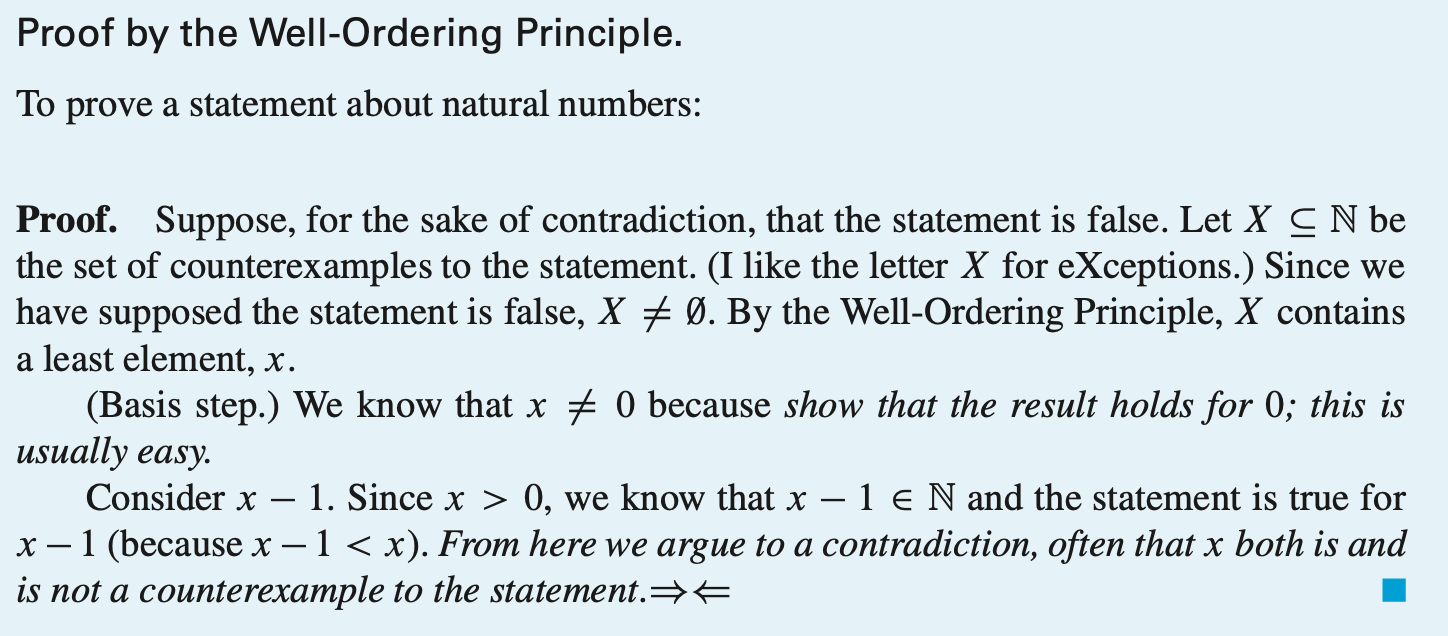
\includegraphics[width=\textwidth]{images/proof_by_well_ordering_principle.png}	
\end{center}
\vfill 
\pause 
\small
\colorbox{blue!30}{\textbf{Remarks.}} 
\begin{itemize}
\item 	The basis step could be a different number than $0$ (e.g. 1) if the statement is about a subset of the natural numbers (e.g. the positive integers).
\item The contradiction needn't come from considering $x-1$.
\end{itemize}

\end{frame}



\begin{frame}[standout]
Group exercises
\end{frame}
\end{document}
